\graphicspath{{chapters/05/images/}}
\chapter{Deterministic simulations}

\section{introduction}
When the last noise term of equation:

$$X(t+\tau)\approx \vec{x}+\sum\limits_{j=1}^Ma_j(\vec{x})\vec{v}_j\tau + \sum\limits_{j=1}^M\sqrt{a_j(\vec{x})\tau}norm(0,1)\vec{v}_j$$

Becomes negligibly small compared with the second done, a deterministic way to computing the dynamics of a system can be applied.
This happens in the limiting case $a_j(\vec{x})\tau\rightarrow\infty$ and the deterministic simulation produces an average behaviour of the system close to the one obtained by averaging an infinite number of stochastic simulations of the system starting from the same initial state.
Deterministic simulation are faster than exact stochastic ones because reaction events are executed as the simultaneous application of a set of reactions.
A single run is sufficient because stochasticity of the system is not considered any more.
One way to simulate a biological system according to a deterministic approach is to translate it into a set of ordinary differential equations or ODEs.

\section{From biochemical reactions to ODEs}
Ordinary differential equations can be used to simulate a biochemical system that satisfied the spatial homogeneity and the continuum hypothesis.

  \subsection{Starting hypothesis}

    \subsubsection{Continuum hypothesis}
    A biochemical system satisfies the continuum hypothesis if the number of molecules for each species is large enough to safely approximate molecular abundances by concentrations that vary continuously.

    \subsubsection{Effect of starting hypothesis}
    Spatial homogeneity allows to randomize spatial information: the rate of each reaction is space independent.
    The continuum hypothesis allows to approximate discrete changes in molecule number by continuous changes in concentration, moreover individual reactions are infinitesimal changes in molecule abundance.
    This holds for species with molecules counts of thousands or more.
    In the cases where molecule abundance is low, its changes will have to be treated like discrete steps in population size and stochastic simulation should be preferred.

  \subsection{Law of mass action}
  When the two hypothesis are satisfied, a biochemical reaction system can be translated inot a set of ODEs by the law of mass action.
  The law of mass action states that the deterministic rate of a chemical reaction is proportional to the product of the concentrations of its reactants.
  Now let $[A] = \frac{\# A}{N_AV}$ be the molar concentration of species $A$ in a chemical volume $V$ and $N_A$ Avogadro's number.
  Some example of conversion of chemical reactions into ODEs are outlined in table \ref{tab:chem-odes}.

  \begin{table}[H]
    \centering
    \begin{tabular}{c c c c}
      \hline
      Reaction type & Reaction & Rate & ODEs\\
      \hline
      Zero-order reaction & $\emptyset\xrightarrow[]{k} A$ & $k$ & $\frac{d[A]}{dt} = k$\\
      First-order reaction & $A\xrightarrow[]{k} B$ & $k[A]$ & $\frac{d[A]}{dt} = -k[A];\frac{d[B]}{dt} = k[A]$\\
      Second-order reaction & $A+B\xrightarrow[]{k} C$ & $k[A][B]$ & $\frac{d[A]}{dt} = \frac{d[B]}{dt} = -k[A][B];\frac{d[C]}{dt} = k[A][B]$\\
      \makecell{Second-order reaction\\ same reactant} & $A+A\xrightarrow[]{k} B$ & $k[A]^2$ & $\frac{d[A]}{dt} = -k[A]^2;\frac{d[B]}{dt} = k[A]^2$\\
      Third-order reaction & $A+B+C\xrightarrow[]{k} D$ & $k[A][B][C]$ & \makecell{$\frac{d[A]}{dt} = \frac{d[B]}{dt} = \frac{d[C]}{dt} =  -k[A][B][C]$\\$\frac{d[D]}{dt} = k[A][B][C]$}\\
      \hline
    \end{tabular}
    \caption{Conversion of biochemical reactions into ODEs}
    \label{tab:chem-odes}
  \end{table}

  Taking into consideration that the deterministic rate $k$ is not the stochastic reaction rate constant $c_j$ but will be computed as in table \ref{tab:chem-rates}.

  \begin{table}[H]
    \centering
    \begin{tabular}{c c c c}
      \hline
      Reaction type & Reaction & Rate & Unit\\
      \hline
      Zero-order reaction & $\emptyset\xrightarrow[]{k} A$ & $k = \frac{c}{N_AV}$ & $concentration\cdot time^{-1}$\\
      First-order reaction & $A\xrightarrow[]{k} B$ &  $k = c$ & $time^{-1}$\\
      Second-order reaction & $A+B\xrightarrow[]{k} C$ & $k = cN_AV$ & $concentration^1time^{-1}$\\
      \makecell{Second-order reaction\\ same reactant} & $A+A\xrightarrow[]{k} B$ & $k = \frac{cN_AV}{2}$ & $concentration^1time^{-1}$\\
      Third-order reaction & $A+B+C\xrightarrow[]{k} D$ & $k = c(N_AV)^2$ & $concentration^2time^{-1}$\\
      \hline
    \end{tabular}
    \caption{Conversion of biochemical reactions into ODEs}
    \label{tab:chem-odes}
  \end{table}

  \subsection{Building the set of ODEs}
  Consider now a biochemical reaction system with $N$ species $S_1, \dots, S_N$ interacting trough $M$ reactions $R_1, \dots R_M$ and a stoichiometric matrix:

  $$\vec{v} = \vec{v}^+-\vec{v}^-$$

  The deterministic rate constant of each reaction is:

  $$k_j = \frac{c_j(N_AV)^{Order_j-1}}{\prod\limits_{i=1}^N\vec{v_{ij}^-!}}$$

  Where $Order_j$ is the order of reaction $R_j$.
  The set of ODEs modelling the evolution of the species is:

  $$\frac{d[S_i]}{dt} = \sum\limits-{j=1}^M\left(k_j\vec{v}_{ji}\prod\limits_{l=1}^N[S_l]^{\vec{v}_{jl}}\right), \forall i = 1, \dots, N$$

  Other methods can be used to approach this translation like the Michaelis-Menten kinetics or the Hill kinetics.
  The former can be used to quantify cooperative binding, the phenomena of binding of a ligand to a macromolecule enhancing when another molecule is attached to the same macro-one.

  \subsection{Michaelis-Menten kinetics}
  Michaelis-Menten (MM) kinetics are used to model enzymatic reactions:

  $$A\xrightarrow[]{E} B$$

  Enzyme accelerate the reaction, and to transform this reaction into a law of mass action it needs to be expanded into:

  $$A+E\xleftrightharpoons[k_2]{k_1} AE\xrightarrow[]{k_3} B+ E$$

  Describing the process more accurately.
  The translation to a set of ODE of the reaction requires the definition of four differential equation, where also $[E]$ and $[EA]$ are considered.
  The MM kinetics allow to simplify the model by reducing the number of equation, so the equation i stranslated into two odes considering the variation of concentration of $A$ and $B$:

  $$\frac{d[A]}{dt} = -\frac{d[B]}{dt} = -V_{MAX}\frac{[A]}{K_M + [A]}$$

  Where:

  \begin{multicols}{2}
    \begin{itemize}
      \item $V_{MAX}$ is the maximum velocity of the enzymatic reaction.
      \item $K_M$, Michaelis constant, is the concentration of the substrate at which the reaction rate is half of its maximum.
    \end{itemize}
  \end{multicols}

  The effect of the enzyme is modelled, where:

  $$K_M = \frac{k_2+k_3}{k_1}\qquad\land\qquad V_{MAX} = k_{cat}[E_T]$$

  Where $[E_T]$ is the enzyme available to the system.
  This kinetics can be used also in the context of stochastic simulation, so that the propensity for this type of reactions will be:

  $$a(\vec{x}) = \frac{V_{MAX}A}{K_M+A}$$

  Where $V_{MAX}$ and $K_M$ are scaled to consider molecule abundances.

\section{Numerical solution of ODEs}
The simulation of a system of ODE is addressed by solving the initial value or Cauchy problem.
This corresponds to finding the solution of a set of differential equations that satisfies the initial condition corresponding to the initial concentration of the species.
An exact solution is usually to complex, so suitable numerical methods need to be used.
This will produce approximations of the solution at specified time points.
Some interpolation methods can be used to obtain intermediate values.
Even when an exact solution if found, the dynamics of the biochemical system is an approximation.

  \subsection{Finding a solution}
  Consider the system with $N$ species:

  $$\frac{d[X]}{dt} = \vec{F}(t,[X])$$

  Where:

  \begin{multicols}{2}
    \begin{itemize}
      \item $\vec{F}:\mathbb{R}\times\mathbb{R}^N\rightarrow\mathbb{R}^N$ is the vector of $N$ functions providing the time derivatives of species concentration.
      \item $[X]$ is the current state of the system expressed in molecular concentrations.
    \end{itemize}
  \end{multicols}

  Let $I = (0,T_{\max})$ be the integration interval of the system and:

  $$t_n = nh, h>0\land n = 0, \dots, N_h$$

  Be the sequence of discretization of $I$ into subintervals $I_n = [t_n, t_{n+1}]$, where:

  \begin{multicols}{2}
    \begin{itemize}
      \item $N_h$ is the maximum integer such that $t_{N_h}\le T_{max}$.
      \item $h$ is the discretization stepsize.
    \end{itemize}
  \end{multicols}

  Numerical methods compute a sequence of states $[X_n]$.
  Approximating the trajectory in terms of concentrations along the time steps starting from $[X_0]$.
  These methods can be explicit or implicit.
  They are called explicit if $[X_{n+1}]$ can be computed directly from the previous state $[X_k]$.
  They are called implicit if $[X_{n+1}]$ depends implicitly on itself through $\vec{F}$.

  \subsection{Forward/Backward Euler method}
  The Forward Euler method is an explicit method, while the backward one is an implicit.
  The are:

  \begin{align*}
    \text{Forward Euler: } [X_{n+1}] &= [X_n] + h\vec{F}(t_n, [X_n])\\
    \text{Backward Euler: } [X_{n+1}] &= [X_n] + h\vec{F}(t_{n+1}, [X_{n+1}])\\
  \end{align*}

  Comparing this with the chemical Langevin equation, when stochasticity is negligible, the CLE reduces a forward Euler with $\tau=h$.

    \subsubsection{Forward Euler algorithm}
    An implementation of the forward Euler algorithm is found in algorithm \ref{algo:forward-euler}.

    \begin{algorithm}[H]
\DontPrintSemicolon
\SetKwComment{comment}{$\%$}{}
\SetKw{Int}{int}
\SetKw{To}{to}
\SetKw{Return}{return}
\SetKw{Not}{not}
\SetKw{Input}{Input}
\SetKw{Output}{Output}
\SetKw{False}{false}
\SetKw{True}{true}
\SetKwData{Item}{item}
\SetKwFunction{Min}{min}
\SetKwFunction{TitleFunction}{Forward Euler method}

\caption{\protect\TitleFunction{}}
\label{algo:forward-euler}

\Input: a system of ODEs $\frac{d[X]}{dt} = \vec{F}(t, [X])$ corresponding to a biochemical reaction system, the initial state $[X_0]$ of the system with species concentrations at time $0$, the simulation ending time $T_{\max}$ and the discretization stepsize $h$\;

\Output: a trajectory of the biochemical system expressed in terms of molecule concentrations with discretization stepsize $h$\;

$t = 0$\;
$[X] = [X_0]$\;


\While{$t<T_{\max}$}{
	$[X] = [X] + h\cdot\vec{f}(t, [X])$\;
	$t = t+h$\;
}
\end{algorithm}


    \subsubsection{Backward Euler algorithm}
    An implementation of the backward Euler algorithm is found in algorithm \ref{algo:backward-euler}.

    \begin{algorithm}[H]
\DontPrintSemicolon
\SetKwComment{comment}{$\%$}{}
\SetKw{Int}{int}
\SetKw{To}{to}
\SetKw{Return}{return}
\SetKw{Not}{not}
\SetKw{Input}{Input}
\SetKw{Output}{Output}
\SetKw{False}{false}
\SetKw{True}{true}
\SetKwData{Item}{item}
\SetKwFunction{Min}{min}
\SetKwFunction{TitleFunction}{Backward Euler method}

\caption{\protect\TitleFunction{}}
\label{algo:backward-euler}

\Input: a system of ODEs $\frac{d[X]}{dt} = \vec{F}(t, [X])$ corresponding to a biochemical reaction system, the initial state $[X_0]$ of the system with species concentrations at time $0$, the simulation ending time $T_{\max}$ and the discretization stepsize $h$\;

\Output: a trajectory of the biochemical system expressed in terms of molecule concentrations with discretization stepsize $h$\;

$t = 0$\;
$[X] = [X_0]$\;


\While{$t<T_{\max}$}{
	estimate $[X_{new}] = [X] + h\cdot\vec{F}(t, [X])$\;
	$t = t+h$\;
	$[X] = [X] + h\cdot\vec{f}(t, [X_{new}])$\;
}
\end{algorithm}


    \subsubsection{Discussion}
    Implicit methods are less intuitive because they need to compute an estimation of the state.
    This can be done by computing a first approximation of the next state which is used then to compute the actual one.



\section{Improving the accuracy of numerical methods}
The accuracy of the computation depends on the discretization stepsize and on the properites of the numerical method.
The general form of one step for an explicit method is:

$$[X_{n+1}] = [X_n] +h\mathbb{F}(t_n, [X_n], \vec{F}(t_n, [X_n])lh) + h\epsilon_{n+1}(h)$$

Where:

\begin{multicols}{2}
  \begin{itemize}
    \item $n = 0, \dots, N_h$.
    \item $h>0$.
    \item $\mathbb{F}$ is the increment function.
    \item $\epsilon_{n+1}(h)$ is the local truncation error LTE at $t_{n+1}$ of the numerical method.
      This provides a measure of how distant the estimation is from the exact value.
  \end{itemize}
\end{multicols}

A global truncation error is required to evaluate the accuracy of a numerical method.

  \subsection{Global truncation error}
  Consider a numerical method with local truncation error $e_{n+1}(h)$.
  The global truncation error is:

  $$\epsilon(h) = \max|\epsilon_{n+1}(h)|, n = 0, \dots, N_h$$

  \subsection{Consistency of a numerical method}
  A numerical method with global truncation error $\epsilon(h)$is consiste with the initial value problem if:

  $$\lim\limits_{h\rightarrow 0}\epsilon(h) = 0$$

  From now on only consistent numerical methods will be considered.

  \subsection{Order of a numerical method}
  A numerical method with global truncation error $\epsilon(h)$ has order $p$ if:

  $$\forall t\in]0, T_{\max}[: \epsilon(h) = O(h^p), h\rightarrow 0$$

  A Taylor expansion shows that the forward Euler has order $1$.
  To increase the accuracy of a simulation the discretization stepsize or increase the order of the numerical methods need to be decreased.
  Decreasing the discretization stepsize implies to compute more simulation steps, while increasing the method order the complexity of each step increases.

  \subsection{Heun method}
  An example of a second order numerical method is the implicit trapezoidal or Crank-Nicolson method, which updates the system by:

  $$[X_{n+1}] = [X_n] + \frac{h}{2}[\vec{F}(t_n, [X_n]) + \vec{F}(t_{n+1}, [X_{n+1}])]$$

  The gain in accuracy is balanced by the increased complexity in the update formula, which requires the evaluation of two $\vec{F}$ at each step.
  This can be transformed into the explicit alternative Heun method, which updates the system by:

  $$[X_{n+1}] = [X_n] + \frac{h}{2}[\vec{F}(t_n, [X_n]) + \vec{F}(t_{n+1}, [X_{n}]+h\vec{F}(t_n, [X_n]))]$$

    \subsubsection{Algorithm}
    An implementation of the Heun algorithm can be found in algorithm \ref{algo:heun}.

    \begin{algorithm}[H]
\DontPrintSemicolon
\SetKwComment{comment}{$\%$}{}
\SetKw{Int}{int}
\SetKw{To}{to}
\SetKw{Return}{return}
\SetKw{Not}{not}
\SetKw{Input}{Input}
\SetKw{Output}{Output}
\SetKw{False}{false}
\SetKw{True}{true}
\SetKwData{Item}{item}
\SetKwFunction{Min}{min}
\SetKwFunction{TitleFunction}{Heun method}

\caption{\protect\TitleFunction{}}
\label{algo:heun}

\Input: a system of ODEs $\frac{d[X]}{dt} = \vec{F}(t, [X])$ corresponding to a biochemical reaction system, the initial state $[X_0]$ of the system with species concentrations at time $0$, the simulation ending time $T_{\max}$ and the discretization stepsize $h$\;

\Output: a trajectory of the biochemical system expressed in terms of molecule concentrations with discretization stepsize $h$\;

$t = 0$\;
$[X] = [X_0]$\;


\While{$t<T_{\max}$}{
  $[X] = [X] + \frac{h}{2}[\vec{F}(t, [X]) + \vec{F}(t, [X]+h\vec{F}(t, [X]))]$\;
	$t = t+h$\;
}
\end{algorithm}


  \subsection{Runge-Kutta methods}
  The Runge-Kutta methods are a family of numerical methods that can be written as:

  $$[X_{n+1}] = [X_n] + h\mathbb{F}(t_n, [X_n], h;\vec{F})$$

  Where:

  \begin{multicols}{2}
    \begin{itemize}
      \item $n = 0, \dots, N_h$.
      \item $h>0$.
      \item $\mathbb{F}$ is the increment function of the method.
    \end{itemize}
  \end{multicols}

  In particular:

  $$\mathbb{F}(t_n, [X_n], h;\vec{F}) = \sum\limits_{i=1}^s b_iK_i$$

  $$K_i = \vec{F}(t_n + c_ih, [X_n] + h\sum\limits_{j=1}^sa_{ij}K_j)$$

  Whit $s$ being the number of stages of the method and $a_{ij}$, $b_i$ and $c_i$ are suitable numbers that characterize the RK method.
  These method can be explicit or implicit depending on the values of $a_{ij}$.
  The Heun method is an explicit RK method, because $a_{12}$ and $a_{22}$ are zeros.
  The number of stages and the order of the methods are related: the minimum number $s_{\min}$ required to get an explicit RK method of corresponding order is described in table \ref{tab:rk-order}

  \begin{table}[H]
    \centering
    \begin{tabular}{c | c c c c c c c c }
      Order & $1$ & $2$ & $3$ & $4$ & $5$ & $6$ & $7$ & $8$\\
      \hline
      $s_{min}$ & $1$ & $2$ & $3$ & $4$ & $6$ & $7$ & $9$ & $11$\\
    \end{tabular}
    \caption{RK order and $s_{min}$ relationship}
    \label{tag:rk-order}
  \end{table}

  $4$ is the maximum number of stages for which the order is not less than $s_{\min}$.
  For this a four-stage explicit RK method is the more convenient way to solve an initial-value problem.

    \subsubsection{Fourth order RK method}
    An example of an update of a fourth order RK method is:

    $$[X_{n+1}] = [X_n] +\frac{h}{6}(K_1+2K_2+2K_3+k_4)$$

    Where;

    \begin{multicols}{2}
      \begin{itemize}
        \item $K_1 = \vec{F}(t_n, [X_n])$.
        \item $K_2 = \vec{F}(t_n+ \frac{h}{2}, [X_n] + \frac{h}{2}K_1)$.
        \item $K_3 = \vec{F}(t_n +\frac{h}{2}, [X_n] + \frac{h}{2}K_2)$.
        \item $K_4 = \vec{F}(t_{n+1}, [X_n] + hK_3)$.
      \end{itemize}
    \end{multicols}

    This is called RK4 and is one of the most used numerical methods for deterministic simulations.

      \paragraph{Algorithm}
      An implementation of the RK4 method can be found at algorithm \ref{algo:rk4}

      
\begin{algorithm}[H]
\DontPrintSemicolon
\SetKwComment{comment}{$\%$}{}
\SetKw{Int}{int}
\SetKw{To}{to}
\SetKw{Return}{return}
\SetKw{Not}{not}
\SetKw{Input}{Input}
\SetKw{Output}{Output}
\SetKw{False}{false}
\SetKw{True}{true}
\SetKwData{Item}{item}
\SetKwFunction{Min}{min}
\SetKwFunction{TitleFunction}{RK4 method}

\caption{\protect\TitleFunction{}}
\label{algo:rk4}

\Input: a system of ODEs $\frac{d[X]}{dt} = \vec{F}(t, [X])$ corresponding to a biochemical reaction system, the initial state $[X_0]$ of the system with species concentrations at time $0$, the simulation ending time $T_{\max}$ and the discretization stepsize $h$\;

\Output: a trajectory of the biochemical system expressed in terms of molecule concentrations with discretization stepsize $h$\;

$t = 0$\;
$[X] = [X_0]$\;


\While{$t<T_{\max}$}{
  $K_1 = \vec{F}(t, [X])$\;
  $K_2 = \vec{F}(t+ \frac{h}{2}, [X] + \frac{h}{2}K_1)$\;
  $K_3 = \vec{F}(t +\frac{h}{2}, [X] + \frac{h}{2}K_2)$\;
  $K_4 = \vec{F}(t+h, [X] + hK_3)$\;
  $[X] = [X] +\frac{h}{6}(K_1+2K_2+2K_3+k_4)$\;
}
\end{algorithm}


\section{Multistep methods}
A numerical method for the approximation of the initial-value problem is a one step method if $\forall n\ge 0$, the computation of $[X_{n+1}]$ depends only on $[X_n]$, otherwise the scheme is called a multistep method.
Multistep (MS) schemes require one functional evaluation at each step and their accuracy can be increased at the expense of increasing the number of steps.
Thy can be implicit or implicit and have an order of accuracy.

  \subsection{Linear multistep numerical method}
  A linear $(s+1)$-step method is a multistep method whose update formula fits the scheme:

  $$[X_{n+1}] = \sum\limits_{j=0}^sa_j[X_{n-j}] + h\sum\limits_{j=0}^sb_j\vec{F}(t_{n-j}, [X_{n-j}]) + hb_{-1}\vec{F}(t_{n+1}, [X_{n+1}])$$

  Where:

  \begin{multicols}{2}
    \begin{itemize}
      \item $n\ge s\ge 0$.
      \item $a_j, b_j$ are numbers that characterize the method.
        When $b_{-1}= 0$ the method is explicit, otherwise implicit.
    \end{itemize}
  \end{multicols}

    \subsubsection{Midpoint method}
    The midpoint method is a second order, two step linear explicit method, which updates the system by:

    $$[X_{n+1}] = [X_{n-1}] + 2h\vec{F}(t_n, [X_n])$$

    They rely on the fact that the formula depend on some previous state of the system to increase accuracy.
    History dependency does not require additional functional evaluation because previous state are stored during the simulation.
    These reduces the simulation runtime, while increasing the complexity in space of the algorithm.
    The length of the time series of states that needs to be stored  depends on the update formula and increases with the order.

      \paragraph{Algorithm}
      An implementation of the midpoint method can be found in \ref{algo:midpoint}

      
\begin{algorithm}[H]
\DontPrintSemicolon
\SetKwComment{comment}{$\%$}{}
\SetKw{Int}{int}
\SetKw{To}{to}
\SetKw{Return}{return}
\SetKw{Not}{not}
\SetKw{Input}{Input}
\SetKw{Output}{Output}
\SetKw{False}{false}
\SetKw{True}{true}
\SetKwData{Item}{item}
\SetKwFunction{Min}{min}
\SetKwFunction{TitleFunction}{Midpoint method}

\caption{\protect\TitleFunction{}}
\label{algo:midpoint}

\Input: a system of ODEs $\frac{d[X]}{dt} = \vec{F}(t, [X])$ corresponding to a biochemical reaction system, the initial state $[X_0]$ of the system with species concentrations at time $0$, the simulation ending time $T_{\max}$ and the discretization stepsize $h$\;

\Output: a trajectory of the biochemical system expressed in terms of molecule concentrations with discretization stepsize $h$\;

$t = 0$\;
$[X_{old}] = [X_0]$\;
$[X] = [X_{old}] + \frac{h}{2}\left[\vec{F}(t,[X_{old}]) + \vec{F}(t+h, [X_{old}] + h\cdot\vec{F}(t, [X_{old}]))\right]$\;
$t = h$\;


\While{$t<T_{\max}$}{
	$[X_{new}] = [X_{old}] + 2h\cdot\vec{f}(t, [X])$\;
	$[X_{old}] = [X]$\;
	$[X] = [X_{new}]$\;
	$t = t+h$\;
}
\end{algorithm}


      \paragraph{Discussion}
      In order to preserve the order of accuracy of the MS algorithm, the one-step method used in the preliminary phase must have at least the same order of the MS method.

    \subsubsection{Simpson method}
    The Simpson method is a two-step implicit linear model which updates the system by:

    $$[X_{n+1}] = [X_{n-1}] + \frac{h}{3}[\vec{F}(t_{n-1}, [X_{n-1}]) + 4\vec{F}(t_n, [X_n]) + \vec{F}(t_{n+1}, [X_{n+1}])]$$

    \subsubsection{General linear multistep algorithm}
    An implementation of a generic $(s+1)$-step method that requires a preliminary phase where a one-step method is used to compute the first $s$ step of the simulation can be found in algorithm \ref{algo:s1-method}

    \begin{algorithm}[H]
\DontPrintSemicolon
\SetKwComment{comment}{$\%$}{}
\SetKw{Int}{int}
\SetKw{To}{to}
\SetKw{Return}{return}
\SetKw{Not}{not}
\SetKw{Input}{Input}
\SetKw{Output}{Output}
\SetKw{False}{false}
\SetKw{True}{true}
\SetKwData{Item}{item}
\SetKwFunction{Min}{min}
\SetKwFunction{TitleFunction}{Linear $(s+1)$-step method}

\caption{\protect\TitleFunction{}}
\label{algo:midpoint}

\Input: a system of ODEs $\frac{d[X]}{dt} = \vec{F}(t, [X])$ corresponding to a biochemical reaction system, the initial state $[X_0]$ of the system with species concentrations at time $0$, the simulation ending time $T_{\max}$ and the discretization stepsize $h$ and the coefficient values $a_j, b_j$\;

\Output: a trajectory of the biochemical system expressed in terms of molecule concentrations with discretization stepsize $h$\;

$t = 0$\;
$[X_{old}] = [X_0]$\;
compute the first $s$ steps of the dynamics by a one-step numerical method of order at least equal to the implemented multistep method\;

\While{$t<T_{\max}$}{
	\If{$b_{-1}\neq 0$}{
		approximate $[X_{t+h}]$\;
	}
  $[X] = \sum\limits_{j=0}^sa_j[X_{n-j}] + h\sum\limits_{j=0}^sb_j\vec{F}(t_{n-j}, [X_{n-j}]) + hb_{-1}\vec{F}(t_{n+1}, [X_{n+1}])$\;
	$t = t+h$\;
}
\end{algorithm}


  \subsection{Adams methods}
  Adams methods are linear multistep methods that update the system state:

  $$[X_{n+1}] = [X_n] + h\sum\limits_{j=-1}^sb_j\vec{F}(t_{n-j}, [X_{n-j}])$$

  Where:

  \begin{multicols}{2}
    \begin{itemize}
      \item $n\ge s\ge 0$.
      \item $b_j$ are numbers that characterize the method.
        $b_{-1} = 0$ implies that the method is explicit and is called the Adams-Bashforth method, when it is implicit is the Adams-Moulton method.
    \end{itemize}
  \end{multicols}

  \subsection{BDF methods}
  BDF methods are implicit linear multistep methods that update the system by:

  $$[X_{n+1}] = \sum\limits_{j=0}^sa_j[X_{n-j}] + hb_{-1}\vec{F}(t_{n+1}, [X_{n+1}])$$

  Where:

  \begin{multicols}{2}
    \begin{itemize}
      \item $n\ge s\ge 0$.
      \item $a_j$ and $b_{-1}\neq 0$ fully characterize the system.
    \end{itemize}
  \end{multicols}




\section{Adaptive methods}

\section{Issues of deterministic simulation}





A \emph{deterministic} way of calculating the dynamics of a system, when the last (noise) term of CLM equation becomes negligibly small compared with the second one, can be applied.
This happens in the limiting case $a_j(\mathbf{x})\tau → \infty$, $j = 1,...,M$, and the deterministic simulation produces an average behaviour of the system that is very close to the one that results by averaging an infinite number of stochastic simulations of the system starting from the same initial state.
If we work in terms of \emph{moles}, we are moving Avogrado numbers; it is not so distant from the reaction size, the assumption is correct enough.
\\
\\
\noindent
The deterministic simulations should give as an output the same result as an average stochastic simulation.
ODEs can be safely used to simulate a biochemical system that satisfies the spatial homogeneity and continuum hypothesis.
  \subsection{Continuum hypothesis}
  ``A biochemical system satisfies the continuum hypothesis if the number of molecules for each species is large enough to safely approximate molecular abundances by concentrations that vary continuously (as opposed to integer- valued molecule counts).''
  Sometimes, models simply use the ODE formalism, regardless of the hypothesis (since the ODE is the only computational framework allowing to reach the end of the simulation).
  \\
  \\
  \noindent
  We are required to apply conversions and derive the ODE according to the following tables.

  \begin{figure}
    \centering
    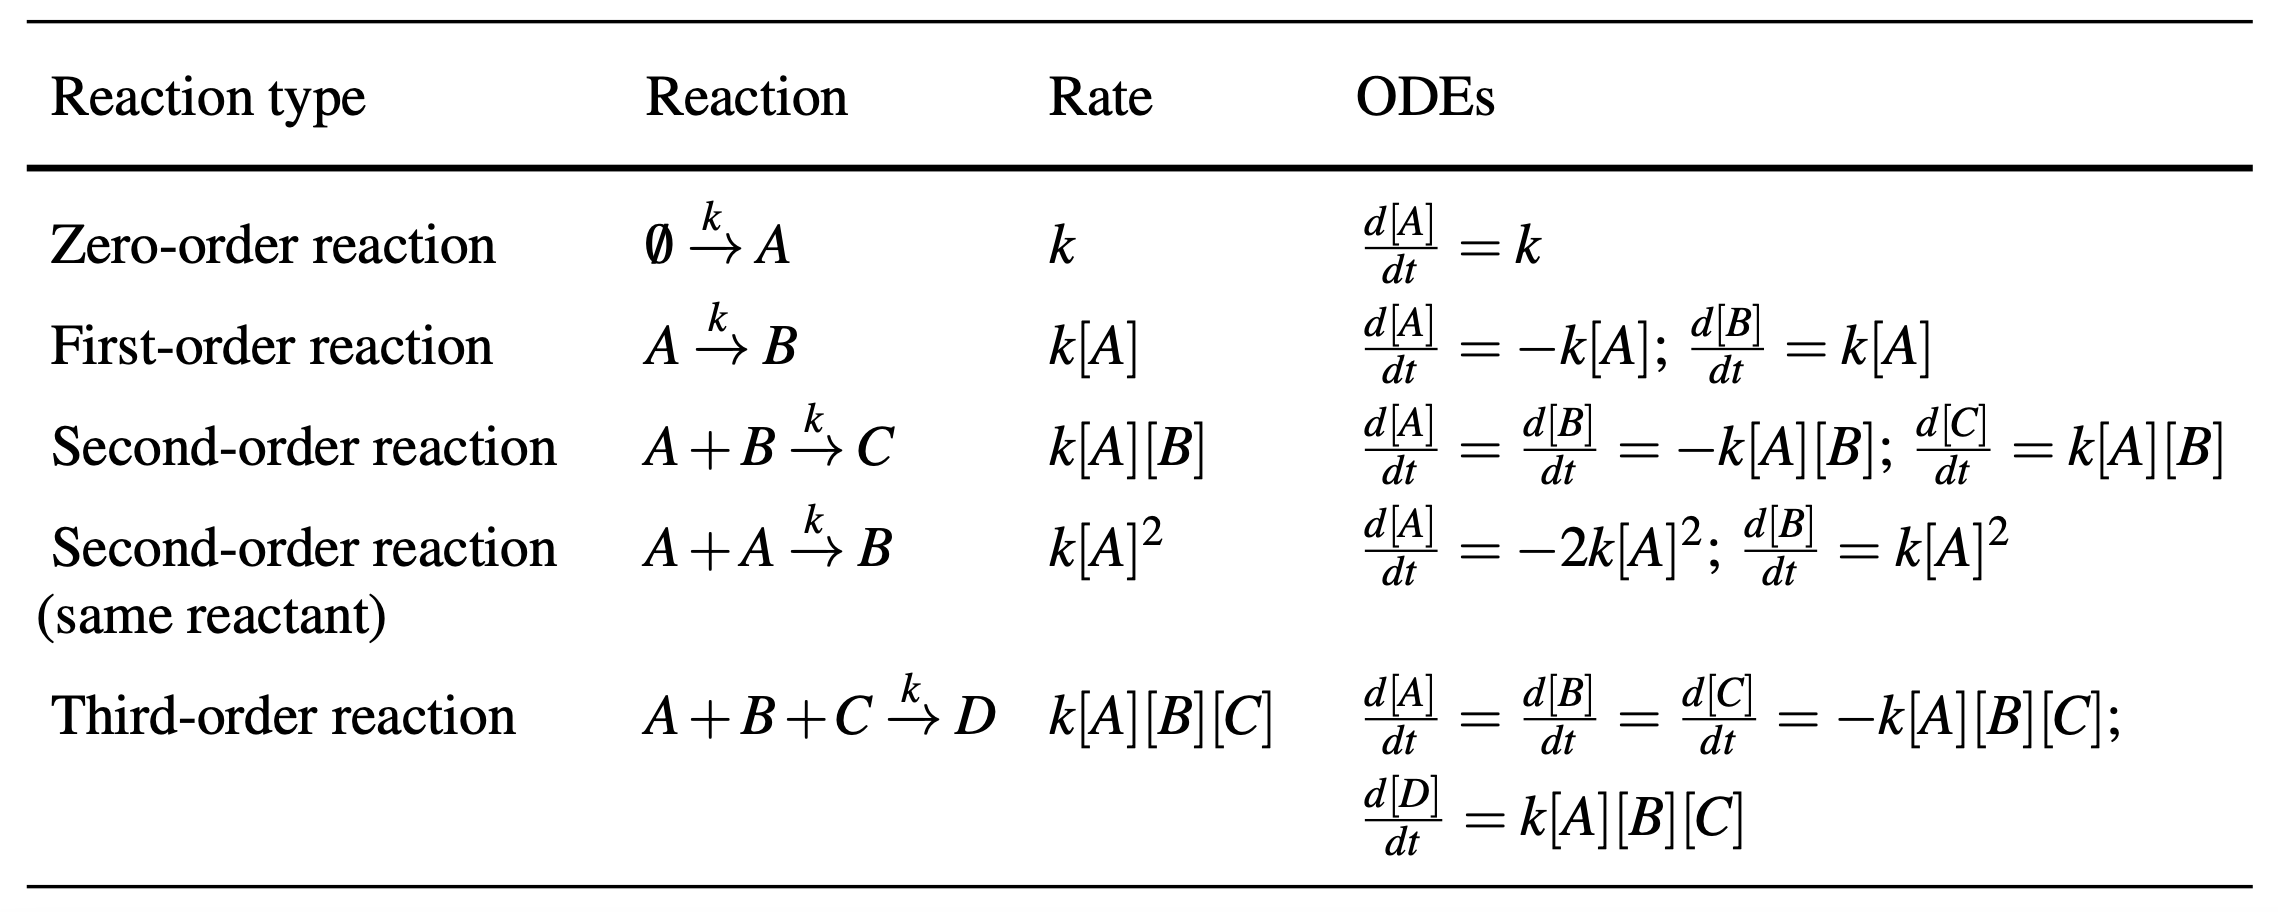
\includegraphics[width=0.5\textwidth]{reaction_ODEs.png}
    \caption{Table 4.4 Marchetti's book}
    \label{fig:rec_ODE}
  \end{figure}

  \noindent
  In Figure \ref{fig:rec_ODE} here we are not considering the combination of the reactants.
  $c$ = stochastic rate, $k$ = deterministic rate.

  \begin{figure}
    \centering
    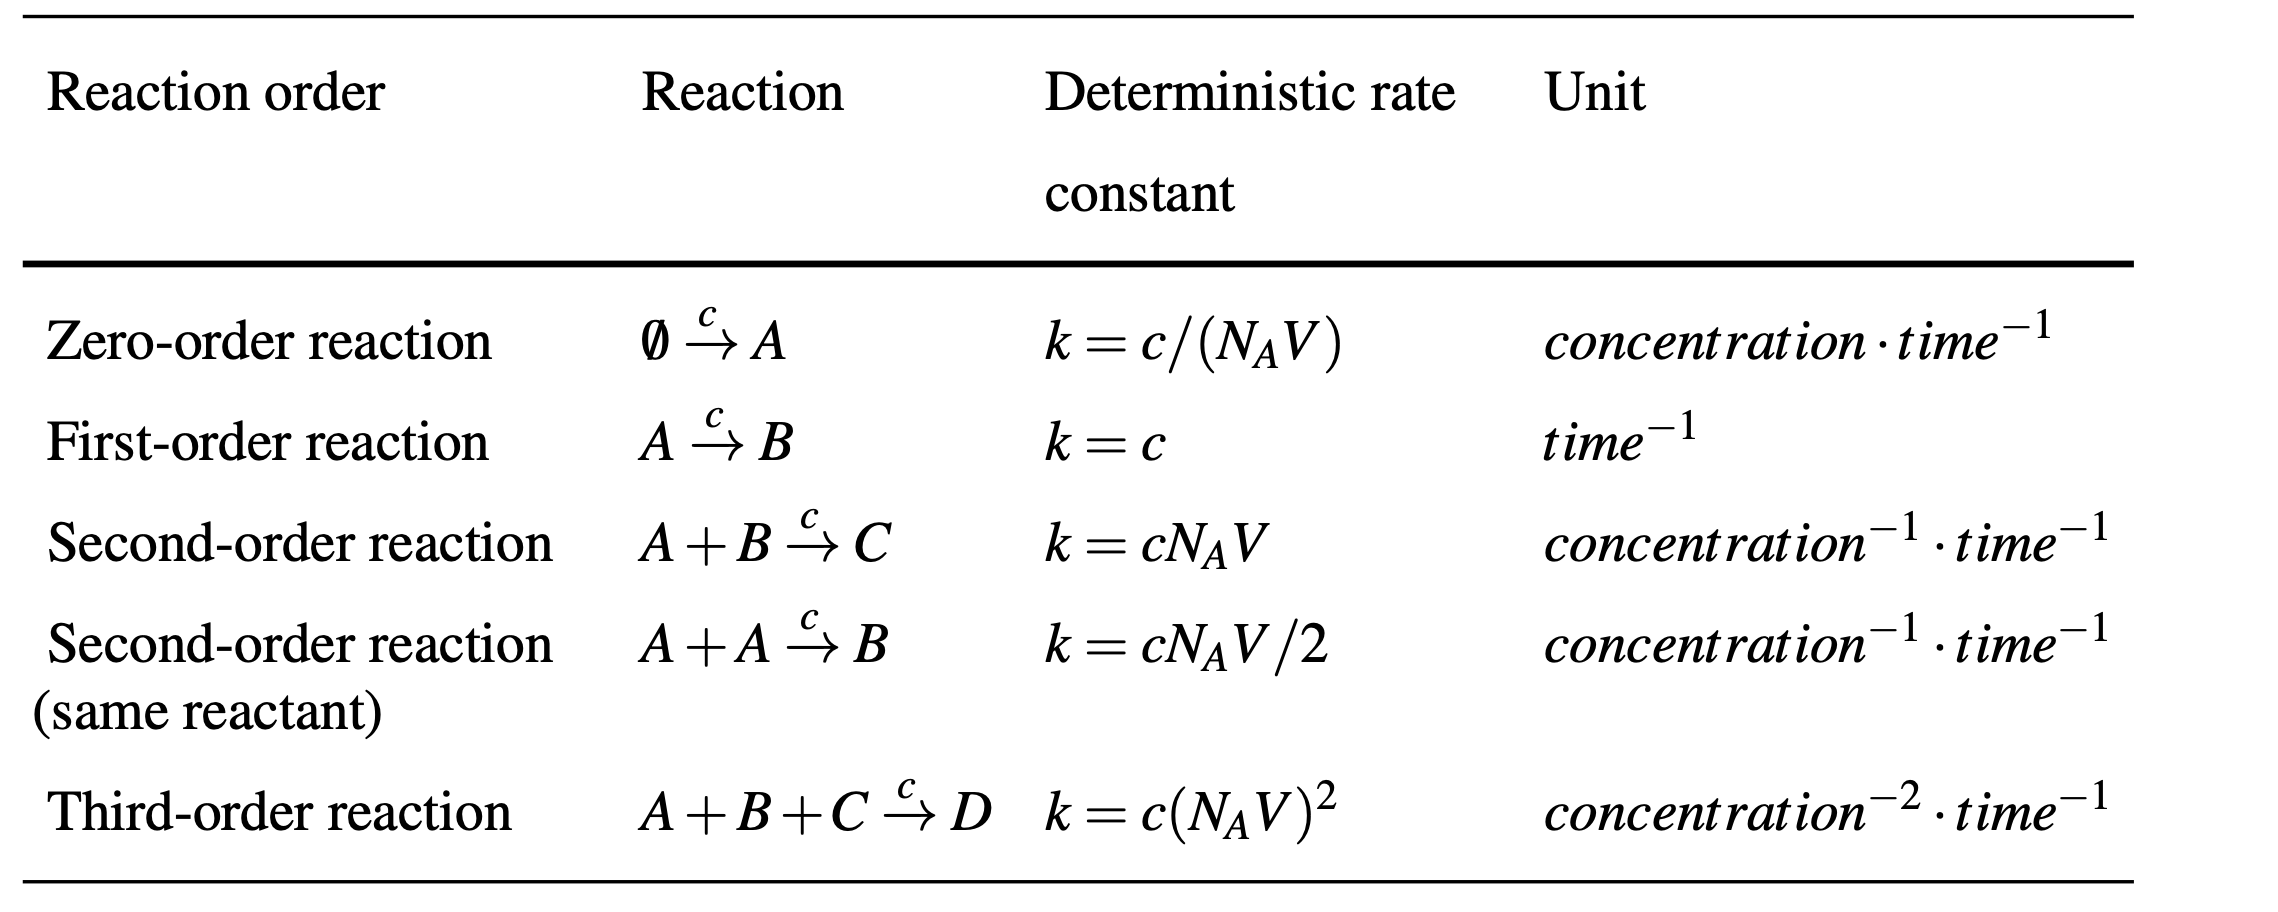
\includegraphics[width=0.5\textwidth]{reaction_rates.png}
    \caption{Table 4.5 Marchetti's book}
    \label{fig:rec_rates}
  \end{figure}

  \noindent
  As shown in Figure \ref{fig:rec_rates} it is possible to go back to the stochastic setting from the deterministic one.
  CLM equation: if we assume that the product is crazily high i.e. ~close to infinite, we can assume that the two parts of the equations have different orders; in this specific condition, the noise part becomes negligible.

\section{Deterministic approximation}
If the propensity is approaching infinite, we can assume that the deterministic setting is motivated.
We are required to introduce the law of mass action and employ tables {[}last lecture{]} to derive a set of ODEs.
In this context, the law of mass action is a bit different from what we have observed at the beginning of the course.
We need to remember that the constant of proportionality, i.e.~rate, is not the same as the stochastic setting.

$$ \frac{d[S_i]}{dt}= \sum^M_{j=1}( k_j\mathbf{v}_{ji}\prod^{N}_{l=1}{[S_l^{\mathbf{v}^{-}_{jl}}]}) ,i = 1,...,N.$$

\noindent
The equation $\frac{d[S_i]}{dt}$ should represent a molar concentration over time.
We have an equation for each of the species $i=1,…,N$.
It should take into consideration the effect of all substances in the system → sum over $M$, considering all reactions, which will be multiplied by the stoichiometric index.
The system is computed as $k$ (constant of proportionality), stoichiometric index and the product of all the reactants.
If a species is not a reactant, $S_i=0$, we end up with 1, only product of the reactants.

$$\frac{d[A]}{dt}= - \frac{d[B]}{dt}= -V_{MAX}\cdot \frac{[A]}{K_M+[A]}$$

\noindent
We can just rely on a simplified set of equations to avid mass action correspondence.
$V_{MAX}$ = maximum velocity of the enzymatic reactions, $K_m$, called \emph{Michaelis constant}, indicates the concentration of the substrate at which the reaction rate is half of its maximum value.

\section{Numerical solution of ODEs}
Often times in computational biology it is unlikely to have enough power for deriving an analytical solution of the system, reality is different and the complexity prevents this kind of approach.
Therefore we rely on numerical methods to compute the simulation, adding an additional layer of approximation.
The algorithm uses the idea of derivative to understand the next value.
For a value of $t>0$, the level of approximation could be remarkable and depends on the dynamics of the system.
Remember that when we simulate in time we have the issue that the computation of the next state depends on the previous state: we are dealing with an iterative formula, so potentially we can have a huge error explosion.
At the basis of such method is the concept of derivative and geometrical rule to identify next step; Euler's method is the simplest one.

  \subsection{Euler's method}
  The first examples of explicit/implicit numerical methods are the \emph{forward Euler method/backward Euler method} for updating the system state:

  \begin{itemize}
    \item Forward Euler: $[X_{n+1}] = [X_n]+h·F(t_n,[X_n])$
    \item Backward Euler: $[X_{n+1}] = [X_n]+h·F(t_{n+1},[X_{n+1}])$
  \end{itemize}
\noindent
  Not surprisingly, for increasing the order of the algorithm we will require a more accurate approx of the derivative, translating in additional evaluation of the ODE.

  \subsection{RUNGE-KUTTA Method}
  RK4 is a 4th order method, good compromise in accuracy and computational requirements.
  This algorithm uses a sort of average over Ks, which are computed by solving the set of ODEs as following:
  $$K1 = F(t_n,[X_n])\\ K2 = F(t_n + 2h,[X_n]+ h2K_1)\\K3 = F(t_n + h2,[X_n]+ h2K_2)\\ K4 = F(t_{n+1},[X_n]+h·K_3)$$.
  Is it possible to increase accuracy without increasing complexity?

  \subsection{Midpoint method}
  2nd order method, we compute the new state at line 5 by two elements: x the current state and x old (the previous one).
  In this case, the multi-step method links the increased order to the number of step previously considered to compute the slope.
  \\
  \\
  \noindent
  Drawback: what happens in the first step? We require an initial state and and additional time series! Limitation of multi-step algorithms: they all require a discretization step, it rules the movement.
  The time should not be computed during the iteration, chosen from the beginning; if we think about this, it can be a limitation of the application of the methodologies, which ask the user an information which might be unknown.
  \\
  \\
  \noindent
  Which is the right time for simulating? Of course we can try to keep the discretization step as small as possible, but the right question that should be asked is: which is the error value? Keeping the error below a certain threshold is not easy, since the dynamics evolve with the system.
  In order to achieve error control, we should apply more requirements to discretization, leading us to seek an \emph{adaptive solution}.
  In order to derive a rough estimate of the error we should compare the state computed by two algorithms of different order: one should be more accurate than the other, to have an idea of the degree of approximation.

  \subsection{Adaptive methods - Runge-Kutta-Fehlberg}
  ``Strapopular algorithm: Runge-Kutta-Fehlberg, RK45 for friends''.
  RK45 is composed of two methods, 4th and 5th order to apply error evaluation {[}4th for dynamics, 5th for estimating the error{]}.
  The algorithm will scale the step (h), in such a way that we keep the deviation below an error threshold.
  A formula will allow to play with h according to the deviation (increase if deviation is little).
  Recall that for the 5th order we require 6 derivations.
  \\
  \\
  \noindent
  The two methods are similar, they share the same Ks, therefore at the price of computing a fifth order method we will have the possibility to obtain two evaluations → quite efficient method.
  ODE45 is this algorithm! Error computation: $\Delta_{n+1}=\frac{|[\tilde{X}*{n+1}]-[X*{n+1}]|}{h}$.
  The error estimate is then compared to the error threshold $\epsilon_t$ provided by the user.
  If $\Delta_{n+1}\leq \epsilon_t$, the local truncation error is assumed to be smaller than the threshold, the state $[X_{n+1}]$ is accepted and the algorithm moves one step forward.
  In the other case, the new state is not accepted and the next state is evaluated again using a different (smaller) value of h.
  In both cases, the value of h is updated as:

  $$h_{n+1}=h_n\sigma \\ \sigma =(\frac{\epsilon_t}{2\Delta_{n+1}})^{1/4}$$

\noindent
  Issue: it's possible that for specific dynamics we will need an infinitesimal $h$ to satisfy the error threshold.
  We can avoid this by updating the strategy, for instance impose an additional threshold to $h$ or insert an heuristic.


\begin{figure}
  \centering
   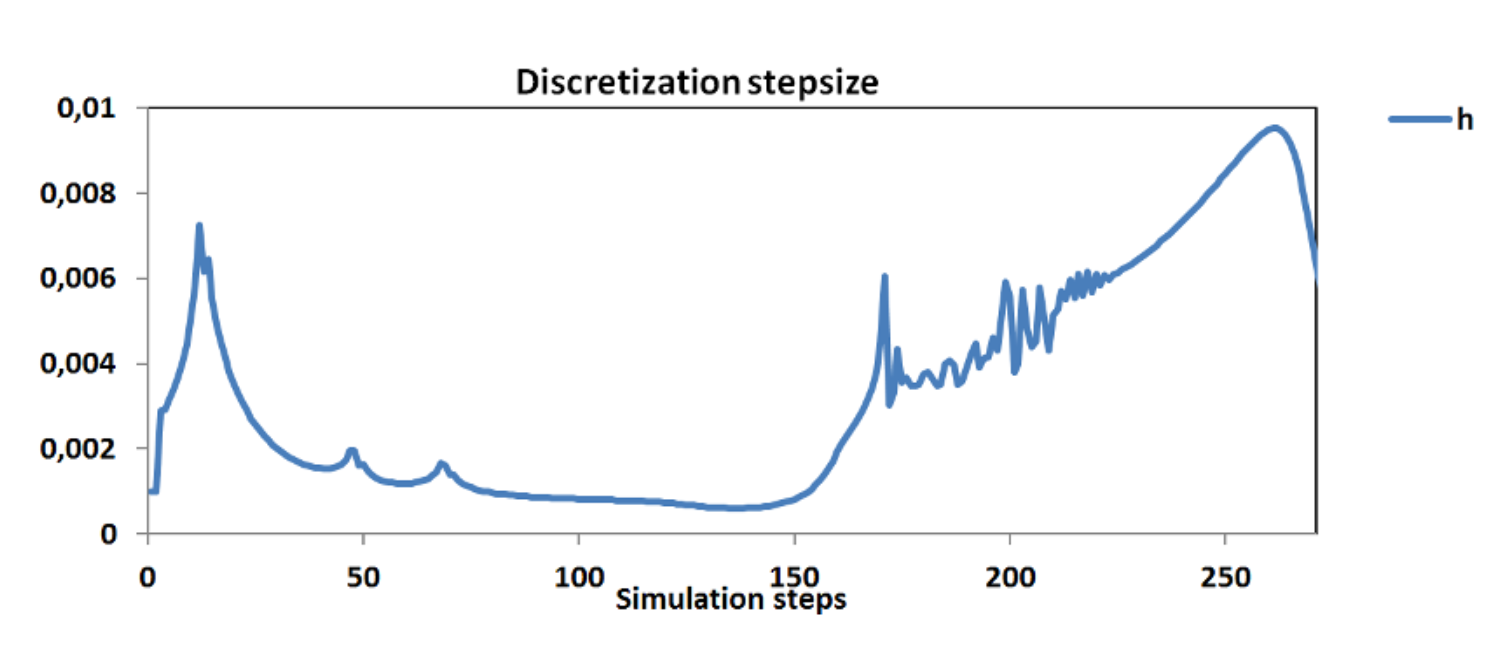
\includegraphics[width=\textwidth]{discretization.png}
  \caption{ Figure 4.9 Marchetti's book}
  \label{fig:discretization}
\end{figure}

  The value of $h$ used at each step is plotted in Figure \ref{fig:discretization}. We can end up in situations in which the system changes a lot → \emph{stiffness condition}, if we work with an adaptive method the property of the dynamics leads to instability in deriving the discretization step.
  Stiffness is a couple property of ODEs and the numerical scheme used to solve the system.
  This means that the same system of ODEs may exhibit stiffness only when it is simulated with some of the numerical schemes introduced in this chapter.
  In MATLAB we can use ODE15S in case of stiffness (happens quite often in biology simulations).
